% This is "sig-alternate.tex" V2.1 April 2013
% This file should be compiled with V2.5 of "sig-alternate.cls" May 2012
%
% This example file demonstrates the use of the 'sig-alternate.cls'
% V2.5 LaTeX2e document class file. It is for those submitting
% articles to ACM Conference Proceedings WHO DO NOT WISH TO
% STRICTLY ADHERE TO THE SIGS (PUBS-BOARD-ENDORSED) STYLE.
% The 'sig-alternate.cls' file will produce a similar-looking,
% albeit, 'tighter' paper resulting in, invariably, fewer pages.
%
% ----------------------------------------------------------------------------------------------------------------
% This .tex file (and associated .cls V2.5) produces:
%       1) The Permission Statement
%       2) The Conference (location) Info information
%       3) The Copyright Line with ACM data
%       4) NO page numbers
%
% as against the acm_proc_article-sp.cls file which
% DOES NOT produce 1) thru' 3) above.
%
% Using 'sig-alternate.cls' you have control, however, from within
% the source .tex file, over both the CopyrightYear
% (defaulted to 200X) and the ACM Copyright Data
% (defaulted to X-XXXXX-XX-X/XX/XX).
% e.g.
% \CopyrightYear{2007} will cause 2007 to appear in the copyright line.
% \crdata{0-12345-67-8/90/12} will cause 0-12345-67-8/90/12 to appear in the copyright line.
%
% ---------------------------------------------------------------------------------------------------------------
% This .tex source is an example which *does* use
% the .bib file (from which the .bbl file % is produced).
% REMEMBER HOWEVER: After having produced the .bbl file,
% and prior to final submission, you *NEED* to 'insert'
% your .bbl file into your source .tex file so as to provide
% ONE 'self-contained' source file.
%
% ================= IF YOU HAVE QUESTIONS =======================
% Questions regarding the SIGS styles, SIGS policies and
% procedures, Conferences etc. should be sent to
% Adrienne Griscti (griscti@acm.org)
%
% Technical questions _only_ to
% Gerald Murray (murray@hq.acm.org)
% ===============================================================
%
% For tracking purposes - this is V2.0 - May 2012

\documentclass{sig-alternate-05-2015}
\usepackage[utf8]{inputenc}

\begin{document}

% Copyright
%\setcopyright{acmcopyright}
%\setcopyright{acmlicensed}
%\setcopyright{rightsretained}
%\setcopyright{usgov}
%\setcopyright{usgovmixed}
%\setcopyright{cagov}
%\setcopyright{cagovmixed}


% DOI
%\doi{10.475/123_4}

% ISBN
%\isbn{123-4567-24-567/08/06}

%Conference
\conferenceinfo{AsianPLoP 2016}{February 24-26, Taiwan.}

%\acmPrice{\$15.00}

%
% --- Author Metadata here ---

%\CopyrightYear{2007} % Allows default copyright year (20XX) to be over-ridden - IF NEED BE.
%\crdata{0-12345-67-8/90/01}  % Allows default copyright data (0-89791-88-6/97/05) to be over-ridden - IF NEED BE.
% --- End of Author Metadata ---

\title{A pattern for Web Browser Infrastructure}
%\subtitle{[Extended Abstract]
%\titlenote{A full version of this paper is available as
%\textit{Author's Guide to Preparing ACM SIG Proceedings Using
%\LaTeX$2_\epsilon$\ and BibTeX} at


\numberofauthors{3} %  in this sample file, there are a *total*
% of EIGHT authors. SIX appear on the 'first-page' (for formatting
% reasons) and the remaining two appear in the \additionalauthors section.
%

\author{
\alignauthor
Paulina Silva\\
  \affaddr{Departamento de Informática}\\
  \affaddr{Universidad Técnica Federico Santa María}\\
  \affaddr{Valparaíso, Chile}\\
  \email{pasilva@alumnos.inf.utfsm.cl}
% 2nd. author
\alignauthor
Raúl Monge\\
  \affaddr{Departamento de Informática}\\
  \affaddr{Universidad Técnica Federico Santa María}\\
  \affaddr{Valparaíso, Chile}\\
  \email{rmonge@inf.utfsm.cl}
% 3rd. author
\alignauthor 
Eduardo B. Fernandez\\
  \affaddr{Department of Computer \(\&\) Electrical Engineering and Computer Science}\\
  \affaddr{Florida Atlantic University}\\
  \affaddr{Florida, USA}\\
  \email{fernande@fau.edu}
}

\maketitle
\begin{abstract}
Currently, most software development is focused in creating systems connected to the Internet, which allows to add functionality within a system and facilities to their \textit{Stakeholders}. This leads to depend on a \textit{web client}, such as \textit{Web Browser}, which allows access to services, data or operations that the system delivers. However, the Internet influences the attack surface of the system, and unfortunately many stakeholders and developers are not aware of the risks to which they are exposed. The lack of security education among software developers and the scarce and scattered documentation for browsers (and standardization) could become a big problem in large architectural developments that depend on browsers to perform their services. A Reference Architecture of the \textit{Web Browser}, using Architectural Patterns, could be a starting point for understanding its security mechanisms and architecture, which interacts with a bigger web system. This would  unify ideas and terminology, giving a holistic view of independent implementation details for both the browser and the system it communicates with. We developed a Browser Infrastructure pattern that describes the infrastructure to allow the communication between a Web Client and a Server in the Internet. With this work we propose an architectural pattern as the first piece of our Reference Architecture for Web Browsers and security concerns.
\end{abstract}


%
% The code below should be generated by the tool at
% http://dl.acm.org/ccs.cfm
% Please copy and paste the code instead of the example below. 
%
\begin{CCSXML}
<ccs2012>
 <concept>
  <concept_id>10010520.10010553.10010562</concept_id>
  <concept_desc>Computer systems organization~Embedded systems</concept_desc>
  <concept_significance>500</concept_significance>
 </concept>
 <concept>
  <concept_id>10010520.10010575.10010755</concept_id>
  <concept_desc>Computer systems organization~Redundancy</concept_desc>
  <concept_significance>300</concept_significance>
 </concept>
 <concept>
  <concept_id>10010520.10010553.10010554</concept_id>
  <concept_desc>Computer systems organization~Robotics</concept_desc>
  <concept_significance>100</concept_significance>
 </concept>
 <concept>
  <concept_id>10003033.10003083.10003095</concept_id>
  <concept_desc>Networks~Network reliability</concept_desc>
  <concept_significance>100</concept_significance>
 </concept>
</ccs2012>  
\end{CCSXML}

\ccsdesc[500]{Computer systems organization~Embedded systems}
\ccsdesc[300]{Computer systems organization~Redundancy}
\ccsdesc{Computer systems organization~Robotics}
\ccsdesc[100]{Networks~Network reliability}




\keywords{Browser, Web Client, Browser Architecture, Reference Architecture, Pattern}

\section*{Introduction}
Patterns are encapsulated solutions to recurrent problems and define a way to express requirements and solutions concisely, as well as providing a communication vocabulary for designers \cite{gamma1994design}. The description of architectures using patterns makes them easier to understand, provides guidelines for design and analysis, and can define a way of making their structure more secure.

Security patterns describe solutions to problems that arise from controlling (stopping or mitigating) a set of specific threats through security mechanisms, defined in a given context. The most common use of security patterns is to help application developers -who are not security experts- to add security in their designs. Patterns of this kind are also used to reinforce a legacy system.

The aim of a Reference Architecture is to provide a guide for developers, who are not security experts, to develop architectures for concrete versions of the system or to extend such system. With the use of architectural patterns we describe the Browser Architecture as a Reference Architecture (RA). An RA is created by capturing the essentials of existing architectures and by taking into account future needs and opportunities, ranging from specific technologies, patterns and business models. It can also be derived from domain models.

A Security Reference Architecture is a Reference Architecture where security services have been added in appropriate places to provide some degree of security for a specific system. The basic approach twe will use to build a Security Reference Architecture is the application of a systematic methodology from \cite{fernandez2006methodology,Fernandez2011,Fernandez2015}, which can be used as a guideline to build secure web browser systems and/or evaluate their security levels. The first step was to build a Reference Anrchitecture in a student work, and now we are trying to improve it using security patterns and misuse patterns. By checking if a threat, expressed as a misuse pattern, can be stopped or mitigated in the security reference architecture, we can evaluate its level of security.

In this work, a Browser Infrastructure Pattern is presented as a first step in to the process of developing a Reference Architecture (RA) and Security Reference Architecture (SRA) for the Web Browser. Threat analysis and security patterns were done in a previous work, we will improve the architecture in the construction of the SRA.

%\section*{Related Work}
 % \subsection*{Reference Architecture of the Browser}
 % We tried to find studies by searching relevant keywords in Scopus or doing a forward snowballing from a work \cite{2005-grosskurth-browser-refarch} we knew. Unfortunately to the date there are a few works related to the construction of a Reference Architecture for the Web Browser.

 % In the study made by Larrondo-Petrie et. at \cite{535061} a web browser analysis is done with the goal of obtaining a Domain Model, and Object Model and a Feature Tree which described the structure and functionality a browser had. The domain, explained in th paper, is a distintive set of objects which act according to rules and policies that characterize the Domain. The used methodology obtains the domain is called Object Oriented Analyis. To identify

 % In addition to identifying these domains they are classified according to their role in the system as: Application Domain, Service Domain, Architecture Domain and Implementation Domain. Object Model serves to provide further details, an overview of the entities in the \textit{Web Browser} and their relationships. The \textit{Feature Tree} provides details on the functional aspects of the application. The proposed model, according to the article, should be useful for software developers who build \textbf{Web-based applications} using the \textit{Browser}. This study is quite far from what we want to do in this work, but it serves to get a background of what is happening in the \textit{Web Browser}, even though the information is very outdated.

 % In the work of Grosskurth et al. \cite{2005-grosskurth-browser-refarch,preprint-Grosskurth-browser-archevol}, a reverse engineering tool is used to obtain a reference architecture at a very high-level on two open-source browsers Mozilla and Konqueror. What it was obtained captured the fundamental subsystems to the same domain systems, as well as the relationships between these subsystems. In this architecture the following subcomponents are identified: User Interface, Data Persistence, Browser Engine, Rendering Engine, Networking, Interpreter of Javascript, XML Parser and Backend Display. It is mentioned that these components are tightly integrated (high coupling) with the Rendering Engine, which makes sense in the single-threaded (monoprocess) architecture that have Mozilla and Konqueror; It is a very common design decision in the \textit{Browser} by that time. 

 % By identifying these components, it is said that this would serve both the design and for the maintenance of a system, because it enhances the understanding to help analyze the trade-off between different design options; or it can also serve as a \textit{template} for new designs. Once the conceptual architecture is extracted, an assessment was initiated to compare the specific architecture of each open-source browser, extracted from the source code, to see how much the conceptual model was closer to reality; Also, the constant comparison allowed to refine the Reference Architecture. Browsers used to validate were: Epiphany, Safari, Lynx, Mosaic and Firefox. While there is quite high-level information about the architecture presented, it does not develop more than the abstraction layer. Also, it seems to appear that it depends on the implementation used in the reverse engineering tool.  

 % The paper \cite{Godfrey2000} made in 2000, describes the experience gained by extending the work described in the TAXFORM project. By using PBS, a tool for reverse engineering, it was extracted the software architecture of the Mozilla browser. This was done in order to understand the structure of its components and create high-level architectural views of the system. 

 % The architectural model obtained contains 11 high-level subsystems, from these those which stood out were the HTML Layout, the implementation of tools and the User Interface code. Also, the study mentions that the architecture has deteriorated significantly in a short period of time (the study is from 2000), and it was not planned carefully from the beginning; part of the blame, the author believes, is a consequence from the \textit{browser wars} in the 90s. While the work helps to understand a little the structure behind the browser, this work is very old and the latest version of the browser has changed considerably. Also, unfortunately the focus of this study does not concern about the internals of th system, but rather the implementation of the reverse engineering tool for the software architecture in a selected browser.

  %Lwin2009 - Agent Based Web Browser
 % In \cite{Lwin2009} proposes a \textit{Browser} called Anfel SOFT, where through the use of Artificial Intelligence, creates agents that improve the user experience. The work ensures that the browser will be able to learn the user's browsing behavior, and guide the user while browsing as effective as possible. The paper obtained the subsystems that can be found in a browser in the same way is done in \cite{2005-grosskurth-browser-refarch}. While the architecture obtained reflects some of what is seen in the 3 browsers chosen in this study, it does not give any details about the identified subsystem. Also, the Reference Architecture obtained is the same as \cite{2005-grosskurth-browser-refarch,preprint-Grosskurth-browser-archevol}, despite identifying other possible components, it adds nothing new.

 % As we already saw in the above studies, some of them build a reference architecture based on reverse engineering techniques. In each work it has been at a very high-level and the description of subcomponents of the system is minimal. Even though they explain the relations between the subsystems, they do not give a better understanding of how they behave in certain situations. In this work is expected explain in more detail the obtained abstractions, including information of the \textit{Browser} use cases as well as the activities carried out with other users. Unfortunately for this study, there is not much literature about the development of a Reference Architecture for \textit{Browser}, and what we found, the most recent work is \cite{Lwin2009} in 2009.

 % \subsection*{Secure Software Development}
 % The literature that concerns of building Secure Software, it indicates that practitioners in software development should understand, largely, the security problems that could potentially arise in their systems. It is not enough to know how to link the pieces together, nor that each piece itself is safe, if the system components do not act in a coordinated way, it probably will not be safe \cite{fernandez2013security}, since security is a systemic property which needs to be seen holistically and the early phases of the software development process.


\section*{Browser Infrastructure Pattern}

  \subsection*{Intent}
  The Browser Infrastructure processes request for a web resource in the Internet for a \textbf{Browser User} (BU), which is a user who uses a browser within a \textbf{Host}. The pattern lets us visualize the communication between the components that make up the Web Browser and the Provider (i.e, a Server), to whom the request is made.

  \subsection*{Example}
  Within the Host is possible that the lack of resources needed to fullfill the user needs are limited. The request of external services or resources is the main reason of the Internet existence. If a user needs to make a bank transaction, such as deposit money to another party, the Browser User will type an URL in the browser to access the online banking service of the bank the user belongs to.
  
  \subsection*{Context}
  Users need to access services or information in the Internet, for which they use specific devices, browsers. A browser starts by receiving a URL from a user and sending it to the corresponding IP address. It also receives the answers that the users want.

  \subsection*{Problem}
  Internet users need resources from Providers, but they may need them in a specific format, for example to be visualized the screen of computer. In this case, if appropiate tools are not available, the resource could not be helpful and it cannot be used correctly. How can the Host and Provider provide these functions? The solution to this problem must resolve the following forces:
  \begin{itemize}
    \item \textit{Transparency}: the user should not be concern about how his request is performed. 
    \item \textit{Stability}: The browser must be capable of working, even if a web page can not be displayed properly or there is an internal problem in the server.
    \item \textit{Isolation}: Each \textit{request} must not interrupt others.
    \item \textit{Heterogeneity}: It does not matter the type of Provider with which the browser communicates, it should be possible to interact with whatever type, and it should be capable of showing the content of the obtained resource adequately.
    \item \textit{Availability}: The user of the Host, should be capable of making a request at any time.
  \end{itemize}

  \subsection*{Solution}
  Provide a device, the Web Browser, with the functions needed to understand user requests and send them to the Provider. A web browser satisfies a request of a Browser User of the Host.

    \subsubsection*{Structure}
    In Figure \ref{fig:BIPatt} the Browser Client (BC) is an entity that represents the main process of a Web Browser, which is constantly communicating with the host of the browser. A Host (H) houses and interacts with the BC. The Host is composed mainly by Hardware (HW), Operative System (OS) and a package to use the Graphic Processing Unit (GPU) to display elements to the Browser User (BU). A user who makes a request to a Internet resources using a Web Browser, will be called Browser User (BU). At the same time, a Provider (P) has HW and OS, and additionally, a Web Server (WS) responsible for receiving external requests. According to the request, a Provider will send the service/resource the Browser User needs. Most Browsers use a central component to do operations that need to affect the Host of the Browser, a Browser Client. Figure \ref{fig:BIPatt} shows the Class diagram for the Browser Infrastructure Pattern. For each new resource a BC requests a created or reused Web Content Renderer (WBR) instance. A Sandbox (S) is created for a single WBR instance, that performs the access control of each communication between the WBR and the BC, as a broker with fine control over the messages (using IPC/IPDL/COM); the same applies to a Plugin (Pl), an Extension (E) and a GPU. Depending on the manufacturer, a Pl could not be Sandboxed. If there is a need for GPU, from Extension and Plugins, they need to communicate directly with the Sandbox which instead will ask for graphical processing.

    \begin{figure*}[h!t]
      \centering
      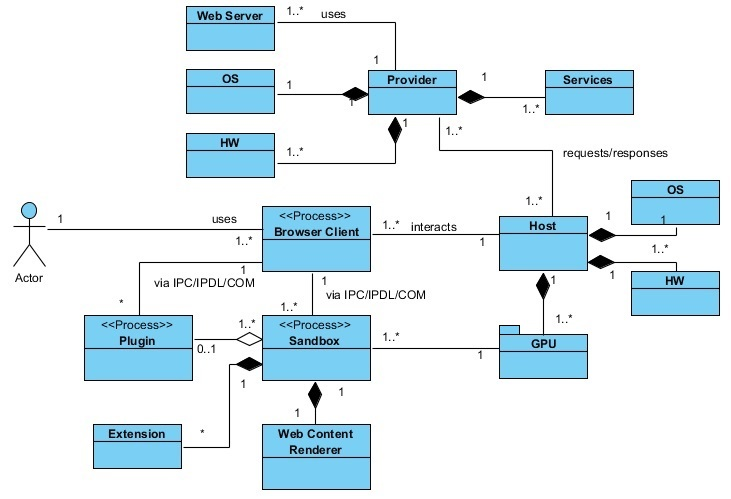
\includegraphics[scale=0.85]{figures/patron_v6.jpg}
      \caption{High-level Components of the Browser Infrastructure.}
      \label{fig:BIPatt}
    \end{figure*}

    \subsubsection*{Dynamics}
    Some use cases are the following:
    \begin{itemize}
      \item Make Request (actor: Browser User)
      \item Cancel Request (actor: Browser User)
      \item Save Resource (actor: Browser User)
      \item Receive Request (actor: Provider)
      \item Ask for Resources (actor: Host)
    \end{itemize}
    We show in detail Make Request below. (Figure \ref{fig:SecReq}):
    \subsubsection*{Summary} A Browser User needs an URL resource which can be obtained by using the HTTP protocol, as required by the Provider. The Browser Client will be used by a User Browser to perform the display of the URL resource.
    \subsubsection*{Actor} Browser User
    \subsubsection*{Preconditions} The Host must have one or more Browser Client for the Host user. In addition to being connected to a network or the Internet. The Provider you want to contact must also be available.
    \subsubsection*{Description}
    Note: Messages between Browser Client and Sandbox can be both synchronous and asynchronous \cite{firefoxIPC,GCIPC}. We do not explain in this work synchronization details, because it is out of our scope. We are interested only in specifying who interacts with whom.
      \begin{enumerate}
        \item A Browser User requires a browser to access a URL for some resource in a Provider, this is done by using a Browser Client already instanced in the Host. With a Sandbox there is an instance of Web Content Renderer pattern.
        \item The Sandbox requires the Host resources to obtain what is behind the URL. A request is made from the Sandbox to the Browser Client through a communication channel such as IPC, IPDL or COM (depending on the \textit{Browser} used) using a limited API to communicate to a process of greater privilege.
        \item The Browser Client receives the request, and verifies through its policy engine if the Sandbox action is allowed.
        \item If the Sandbox action is allowed to obtain a host resources (via system calls), the Network API is used. The Browser Client communicates internally with the Host, and the latter must review its policies to ensure that the Browser Client has the privilege of making a request to the Host resources.
        \item If access to the resource is allowed, the Browser Client may \textit{request} through the Network API. If the \textit{request} is not \textit{pre-flight}, the Provider will receive the \textit{request} and work on it.
        \item The Provider will send a \textit{response} to the \textit{request} received. Depending on how it is implemented the Browser Client, it may or may not have to wait for the response (synchronous or asynchronous) of the Provider.
        \item Once the response is obtained, is stored in the cache, unless it is specified in another way.
        \item The response to the \textit{request} is sent by a communication channel to the Sandbox of origin and then the Web Content Renderer. If a response was received by the \textit{request}, the Web Content Renderer is ready to prepare the parsing of the content or use a plugin or GPU to support the display of the resources obtained by the URL. Otherwise, the Web Content Renderer within the Sandbox will create an error page.
        \item The \textit {Renderer} obtains a bitmap to be sent to the Client Browser, so that the Host can present it. Before doing this, the BC should check that the Sandbox that hosts the Web Content Renderer possesses the permissions to do so.
        \item If the permissions are sufficient, the Browser Client sends the bitmap, as a parameter, in the system call made to the Host. Finally, the Host must check that the system call made by the Browser Client has the proper permissions.
      \end{enumerate}
    \subsubsection*{Alternative flow} 
    \begin{itemize}
    \item The Provider is not available.
    \item The resource pointed by the URL does not exists.
    \item The request is cancelled.
      \end{itemize}
    \subsubsection*{Postconditions} The \textit{Browser} receives the resource indicated by the URL and it is displayed by the peripheral device output for the Browser User.
      \begin{figure*}[h!t]
          \centering
          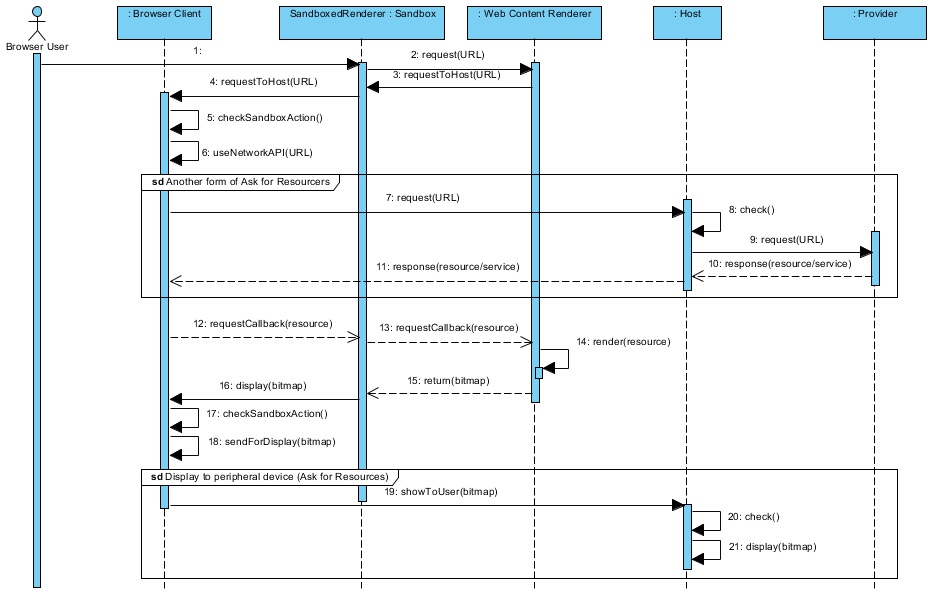
\includegraphics[scale=0.7]{figures/MakeRequest.jpg}
          \caption{Sequence Diagram: Make Request.}
          \label{fig:SecReq}
      \end{figure*}

  \subsection*{Implementation}
  \begin{itemize}
    \item The sandbox may be implemented in various ways. Google Chrome \cite{sandboxGC} is based on not reinventing the wheel and use the protection mechanisms provided by the OS (e.g, Windows or Linux) of the Host to protect the user. This prevents any process to access the file system, and having a restrictive API in the web Content Renderer. Google Chrome, Firefox and Internet Explorer affirm that Sandboxes are an important piece to the Browser because realizes the principle of least privilege \cite{Yason,sandboxGC,sandboxFirefox}. The minimum configuration for the Sandbox includes 2 processes: The privileged process or Broker represented by the Browser Client and the processes hosted by Sandboxes or targets.
    \item To enforce the Same Origin Policy, Google Chrome, Firefox and Internet Explorer use different schemes; for example Google Chrome leaves pages/resources isolated with the help of the Renderer (Web Content Renderer in this case).
  \end{itemize}

  \subsection*{Consequences}
  The Browser Infrastructure pattern provides the following benefits:
  \begin{itemize}
    \item Transparency: The user navigation is done almost automatically, only in rare cases the user will have to make a decision on the resource asked.
    \item Stability: Because the Browser Client, Sandbox, and GPU  Plugin are independent Host processes, the failure of one will not generate problems in other (crash, memory corruption, etc.).
    \item Isolation: Depending on the type of isolation you can separate the different request, so they do not interfere with each other, unless it is desired.
    \item Heterogeneity: Because each Browser Client tries to follow the standards of the W3C \cite{w3c}, every page that follows these guidelines can be viewed, as well as other resources.
    \item Availability: Each process is independent and has its own thread of execution, these were specifically created to help maintain the User Interface smooth.
  \end{itemize}
  At the same time, this pattern has the following liabilities:
  \begin{itemize}
    \item Since independent processes are used to browse a resource (depending on the scheme using the browser), it is possible that a lot of the host's resources are used to keep everything open.
    \item The resources of Providers who have not met the specifications of the W3C, will be display incorrectly by the Web Browser.
  \end{itemize}

  \subsection*{Example Resolved}
With the given pattern it is now possible to navigate smoothly to all resources on the Internet we want. It is possible to provide through the isolation of the components: speed, security and stability. The Browser User will only concern about the navigation, unless it is required for its explicit permission to enter certain Host resources that are privileged (e.g, the file system). Each Host user can use the Browser Client they want, because each one is isolated by using separate processes.
  \subsection*{Known Uses}
  \begin{itemize}
    \item Currently, the separation of the components of the \textit{Browser} in various processes, with different levels of access, is called as Modular Architecture \cite{Vrbanec2013}. This enables the separation of concerns in the browser, which gives greater stability, isolation, safety and speed.
    \item Google Chrome is based on the modular architecture, where each Renderer Process communicates with the Browser Kernel \cite{multiProcGC}. This proposal is used as a reference in the Mozilla project Electrolysis, as you can see in \cite{FirefoxThreatModel,featuresE10S}, specially in the development of the sandbox and architecture.
    \item Internet Explorer, a proprietary browser, does not give much information about its structure or details of its implementation; \cite{Crowley2010} addresses Loosely-Coupled architecture \cite{IE8-LCIE} and its components, but without giving further details. 
    \item Firefox, meanwhile has two implementations: monoprocess and multiprocess/modular. Electrolysis is the name of the modular architecture being implemented, but it has not yet been fully completed.
  \end{itemize}

  \subsection*{Related Patterns}
  \begin{itemize}
    \item The Web Content Renderer pattern, which is under development, represents the subsystem hosted by a Sandbox that allows the parsing of a resource obtained through a request.
    \item The Browser Kernel pattern, a pattern we are developing, represents the subsystem that represents the Web browser central component. This acts as a Reference Monitor pattern \cite{fernandez2013security} for all requests the Renderer does.
    \item The Sandbox is another name for the pattern Controlled Execution Domain \cite{fernandez2013security}.
  \end{itemize}

\section*{Conclusions and Future Work}
A Web browser appears to be a medium complexity software for users and developers without security experience, but unfortunately this piece of software allows a variaty of attack vectors, to the user using it as well as the system with which interacts. Therefore it is important to understand its structure and how it interacts with internal and/or external Stakeholders.

A part of our Reference Architecture has been built through the abstraction of documentation through the Browser Infrastructure pattern. We created our first architectural pattern for the infrastructure of \textit{Web Browser} to help others understand, holistically, the components, interactions and relationships of this system. Furthermore, it has been possible to characterize the Stakeholders and one of the most important use case. From what we have known, this is the second Reference Architecture for the \textit{Browser} built \cite{2005-grosskurth-browser-refarch}. The proposed work allows a better understanding of this system called Web Browser by using our partially Reference Architecture, this is also helpful to understand existing threats. Also, as it is not subject to specific implementations, it is possible to generalize certain results in other browsers.

Future work will be related to the creation of a Security Reference Architecture for the \textit{Web Browser} using the same methodology presented here. Other patterns related to Browser Infrastructure pattern will be obtained in order to complete the RA we already begun, such as the Web Content Renderer and Browser Kernel pattern. An example of the type of work to be carried out can be seen in \cite{Fernandez2015}. This study was focused on carry out activities to build secure software and evaluate the safety levels of a system already built.

We plan to build more Misuse Patterns for the Browser Infrastructure Pattern, to continue the study of the possible threats in the \textit{Browser}, as a way to educate Developers and Stakeholders. At the same time, these patterns will allow the construction of the Security Reference Architecture for the browser. In the same line, in addition to finding potential threats existing in the system, we need to find countermeasures or security defenses to prevent or foresee such threats through security patterns on the reference architecture built.

\bibliography{refTodas}  
\bibliographystyle{IEEEtran}


\end{document}
